\documentclass{beamer}
\mode<presentation>
\usepackage{amsmath}
\usepackage{amssymb}
%\usepackage{advdate}
\usepackage{adjustbox}
\usepackage{subcaption}
\usepackage{enumitem}
\usepackage{multicol}
\usepackage{mathtools}
\usepackage{listings}
\usepackage{xcolor}

\definecolor{mygray}{rgb}{0.5,0.5,0.5}
\definecolor{mymauve}{rgb}{0.58,0,0.82}
\definecolor{myblue}{rgb}{0.13,0.13,0.6}

\lstset{
	language=Python,
	backgroundcolor=\color{white},
	commentstyle=\color{mygray},
	keywordstyle=\color{myblue},
	numberstyle=\tiny\color{mygray},
	stringstyle=\color{mymauve},
	basicstyle=\ttfamily\small, % Change font size here
	breaklines=true,
	numbersep=8pt,
	showstringspaces=false,
	tabsize=4
}
\usepackage{url}
\def\UrlBreaks{\do\/\do-}
\usetheme{Boadilla}
\usecolortheme{lily}
\setbeamertemplate{footline}
{
  \leavevmode%
  \hbox{%
  \begin{beamercolorbox}[wd=\paperwidth,ht=2.25ex,dp=1ex,right]{author in head/foot}%
    \insertframenumber{} / \inserttotalframenumber\hspace*{2ex} 
  \end{beamercolorbox}}%
  \vskip0pt%
}
\setbeamertemplate{navigation symbols}{}

\providecommand{\nCr}[2]{\,^{#1}C_{#2}} % nCr
\providecommand{\nPr}[2]{\,^{#1}P_{#2}} % nPr
\providecommand{\mbf}{\mathbf}
\providecommand{\pr}[1]{\ensuremath{\Pr\left(#1\right)}}
\providecommand{\qfunc}[1]{\ensuremath{Q\left(#1\right)}}
\providecommand{\sbrak}[1]{\ensuremath{{}\left[#1\right]}}
\providecommand{\lsbrak}[1]{\ensuremath{{}\left[#1\right.}}
\providecommand{\rsbrak}[1]{\ensuremath{{}\left.#1\right]}}
\providecommand{\brak}[1]{\ensuremath{\left(#1\right)}}
\providecommand{\lbrak}[1]{\ensuremath{\left(#1\right.}}
\providecommand{\rbrak}[1]{\ensuremath{\left.#1\right)}}
\providecommand{\cbrak}[1]{\ensuremath{\left\{#1\right\}}}
\providecommand{\lcbrak}[1]{\ensuremath{\left\{#1\right.}}
\providecommand{\rcbrak}[1]{\ensuremath{\left.#1\right\}}}
\theoremstyle{remark}
\newtheorem{rem}{Remark}
\newcommand{\sgn}{\mathop{\mathrm{sgn}}}
\providecommand{\abs}[1]{\left\vert#1\right\vert}
\providecommand{\res}[1]{\Res\displaylimits_{#1}} 
\providecommand{\norm}[1]{\lVert#1\rVert}
\providecommand{\mtx}[1]{\mathbf{#1}}
\providecommand{\mean}[1]{E\left[ #1 \right]}
\providecommand{\fourier}{\overset{\mathcal{F}}{ \rightleftharpoons}}
%\providecommand{\hilbert}{\overset{\mathcal{H}}{ \rightleftharpoons}}
\providecommand{\system}{\overset{\mathcal{H}}{ \longleftrightarrow}}
	%\newcommand{\solution}[2]{\textbf{Solution:}{#1}}
%\newcommand{\solution}{\noindent \textbf{Solution: }}
\providecommand{\dec}[2]{\ensuremath{\overset{#1}{\underset{#2}{\gtrless}}}}
\newcommand{\myvec}[1]{\ensuremath{\begin{pmatrix}#1\end{pmatrix}}}
\newcommand{\mydec}[1]{\ensuremath{\begin{vmatrix}#1\end{vmatrix}}}
\let\vec\mathbf

\lstset{
%language=C,
frame=single, 
breaklines=true,
columns=fullflexible
}

\numberwithin{equation}{section}

\title{NCERT: 9.5.7}
\author{Y Siddhanth \\ EE24BTECH11059\\ EE1030}

\date{\today} 
\begin{document}

\begin{frame}
\titlepage
\end{frame}

\section*{Outline}
\begin{frame}
\tableofcontents
\end{frame}
\section{Problem}
\begin{frame}
\frametitle{Problem Statement}
Solve the below differential equation such that the function passes through $\brak{1,1}$.\[
\left\{ x \cos\left(\frac{y}{x}\right) + y \sin\left(\frac{y}{x}\right) \right\} y \, dx = 
\left\{ y \sin\left(\frac{y}{x}\right) - x \cos\left(\frac{y}{x}\right) \right\} x \, dy
\]
\end{frame}

\section{Solution}
\subsection{Theoretical Solution}
\begin{frame}
	\frametitle{Theoretical Solution}
	\begin{align}
		\left\{ x \cos\left(\frac{y}{x}\right) + y \sin\left(\frac{y}{x}\right) \right\} y \, dx &= 
		\left\{ y \sin\left(\frac{y}{x}\right) - x \cos\left(\frac{y}{x}\right) \right\} x \, dy \\ 
		\frac{dy}{dx} &= \frac{ \brak{x \cos\left(\frac{y}{x}\right) + y \sin\left(\frac{y}{x}\right) }y}{\brak{y \sin\left(\frac{y}{x}\right) - x \cos\left(\frac{y}{x}\right) }x} \\
		\frac{dy}{dx} &= \frac{ \brak{x \cos\left(\frac{y}{x}\right) + y \sin\left(\frac{y}{x}\right) }y}{\brak{y \sin\left(\frac{y}{x}\right) - x \cos\left(\frac{y}{x}\right) }x}
	\end{align}
	Taking $v = \frac{y}{x} \implies \frac{dy}{dx} = v + x\frac{dv}{dx}$ and simplifying
	
	\begin{align}
		\frac{dy}{dx} &= \frac{ \brak{1 + v \tan\brak{x} }v}{\brak{v \tan\brak{v} - 1 }}\\
		v + x\frac{dv}{dx} &= \frac{ \brak{1 + v \tan\brak{x} }v}{\brak{v \tan\brak{v} - 1 }}\\
		x\frac{dv}{dx} &= \frac{ 2v}{\brak{v \tan\brak{v} - 1 }}
	\end{align}
\end{frame}
\begin{frame}
	\frametitle{Theoretical Solution}
	\begin{align}
				2\int\frac{dx}{x} &=  \int\tan\brak{v}dv - \int\frac{dv}{v}
	\end{align}
	Solving the integral, we get
	\begin{align}
		2\log\brak{x} + \log{\brak{v}} &= \log|sec{\brak{v}|} + c \\
		2\log\brak{x} + \log{\brak{\frac{y}{x}}} &= \log\abs{sec{\brak{\frac{y}{x}}}} + c \\
		\log{\brak{xy\abs{\cos\brak{\frac{y}{x}}}}} &= c\\
	\end{align}
	Substituting the given conditions,
	\begin{align}
		e^c &= 0.54
	\end{align}
	The theoretical solution is,
	\begin{align}
		xy\abs{\cos\brak{\frac{y}{x}}} &= 0.54
	\end{align}
\end{frame}
\subsection{Numerical Solution}
\begin{frame}
\frametitle{Numerical Solution}
	The numerical solution for this differential equation can be found using the method of Finite Differences \eqref{finited} involving multiple varied stepsizes, bounded (x,y) coordinates and bounded derivative value.
	\begin{align}
		\frac{dy}{dx} &= \frac{y\brak{x+h} - y\brak{x}}{h} \\
		\implies y\brak{x+h} &= y\brak{x} + h\cdot\frac{dy}{dx} \label{finited}
	\end{align}
	Substituting $\frac{dy}{dx}$ into \eqref{finited}, we get
	\begin{align}
		\implies y(x+h) &= y(x) + h\cdot\frac{ \brak{x \cos\left(\frac{y}{x}\right) + y \sin\left(\frac{y}{x}\right) }y}{\brak{y \sin\left(\frac{y}{x}\right) - x \cos\left(\frac{y}{x}\right) }x} 
	\end{align}
\end{frame}
\begin{frame}
	\frametitle{Numerical Solution}
	The numerical solution for this differential equation can be found using the method of Finite Differences \eqref{finited} involving multiple varied stepsizes, bounded (x,y) coordinates and bounded derivative value.
	\begin{align}
		\frac{dy}{dx} &= \frac{y\brak{x+h} - y\brak{x}}{h} \\
		\implies y\brak{x+h} &= y\brak{x} + h\cdot\frac{dy}{dx} \label{finited}
	\end{align}
	Substituting $\frac{dy}{dx}$ into \eqref{finited}, we get
	\begin{align}
		\implies y(x+h) &= y(x) + h\cdot\frac{ \brak{x \cos\left(\frac{y}{x}\right) + y \sin\left(\frac{y}{x}\right) }y}{\brak{y \sin\left(\frac{y}{x}\right) - x \cos\left(\frac{y}{x}\right) }x} 
	\end{align}
\end{frame}
\begin{frame}
	\frametitle{Numerical Solution}
	By using this method iteratively $\brak{x \implies x_n \text{ and } x+h \implies x_{n+1}}$, we can numerically find all the points lying on the curve. The accuracy can be controlled by varying the stepsize or $h$.
	\begin{align}
		y_{n+1} &= y_n + h\cdot\frac{ \brak{x_n \cos\left(\frac{y_n}{x_n}\right) + y_n \sin\left(\frac{y_n}{x_n}\right) }y_n}{\brak{y_n \sin\left(\frac{y_n}{x_n}\right) - x_n \cos\left(\frac{y_n}{x_n}\right) }x_n} 
	\end{align}
\end{frame}
\begin{frame}
	%\frametitle{Numerical Solution}
	\begin{figure}[h]
		\centering
		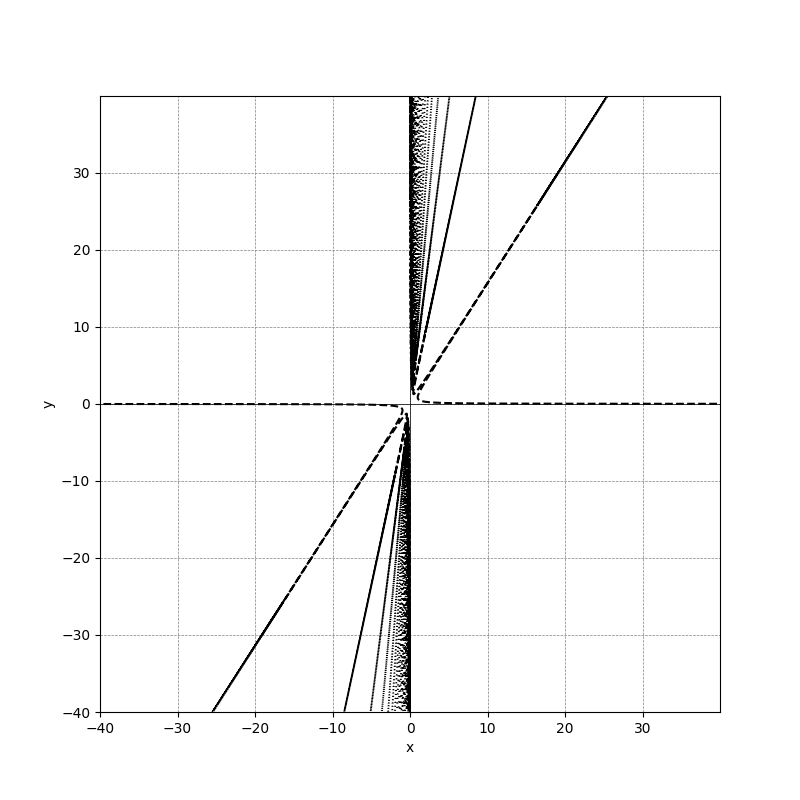
\includegraphics[width=0.8\linewidth]{figs/figo.png}
		\caption{}
		\label{graph3}
	\end{figure}
\end{frame}
\begin{frame}
	\frametitle{Strategy Employed}
	Clearly, this method, with a single step, fails to plot the entire curve when there are multiple branches, discontinuities, or infinite gradients. In this specific problem, the plot consists of an infinite number of skewed hyperbolas, which are impossible to capture using the simple finite differences method.  \\
	This limitation can be addressed by employing multiple step sizes. A large step is initially taken from \(x_0 \to x_1\) (\(h_1\)), and then the points between them are filled using smaller steps (\(h_2 = 0.01\)) in both forward and backward directions. The large steps are taken in a backward direction, where points approach the origin, with step sizes varying from \(0.1 \to 1\), incremented by \(0.001\). Finally, a gradient limit is introduced to avoid infinite gradients and stationary points.  
	
	While this approach has limitations near the \(x\)-axis due to the varying large steps approaching the origin, it performs well as the distance from the origin increases.
\end{frame}
\begin{frame}
	\begin{figure}[h]
		\centering
		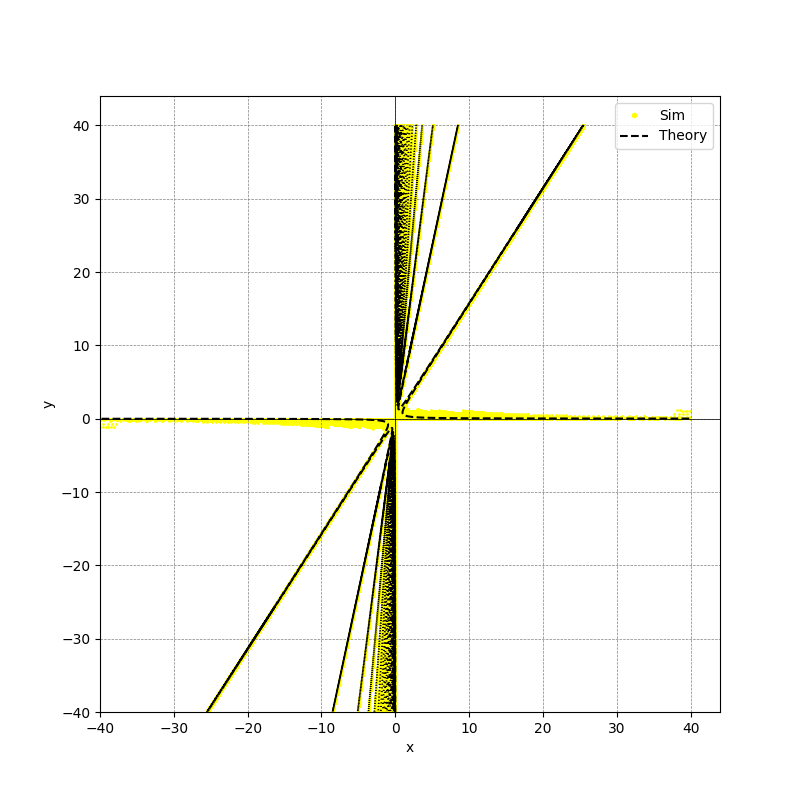
\includegraphics[width=0.8\linewidth]{figs/fig.png}
		\caption{}
		\label{graph3}
	\end{figure}
\end{frame}
\begin{frame}
	\begin{figure}[h]
		\centering
		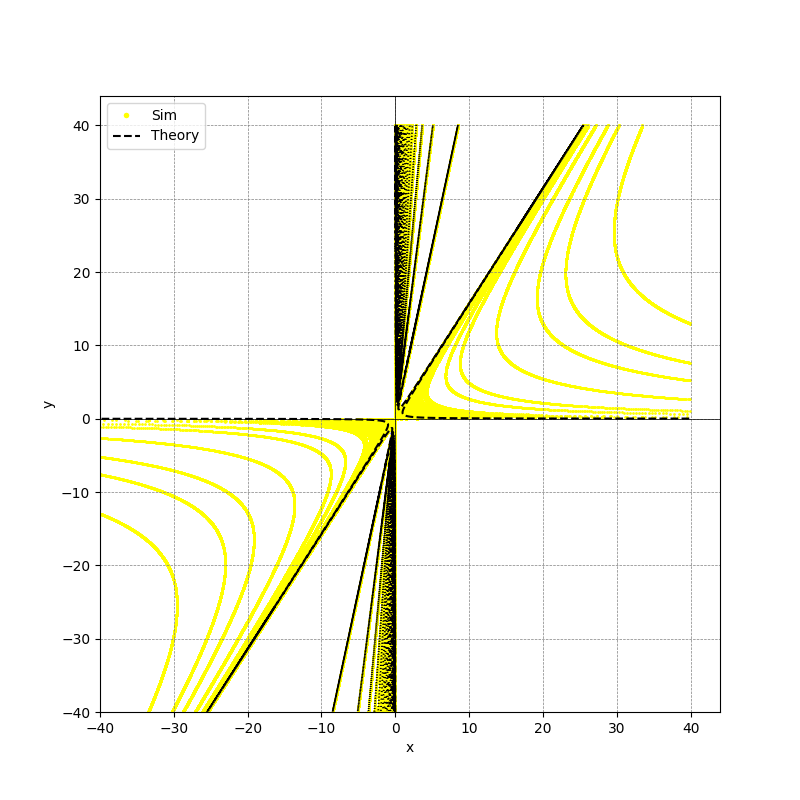
\includegraphics[width=0.8\linewidth]{figs/figf.png}
		\caption{}
		\label{graph3}
	\end{figure}
\end{frame}
\begin{frame}
	\begin{figure}[h]
		\centering
		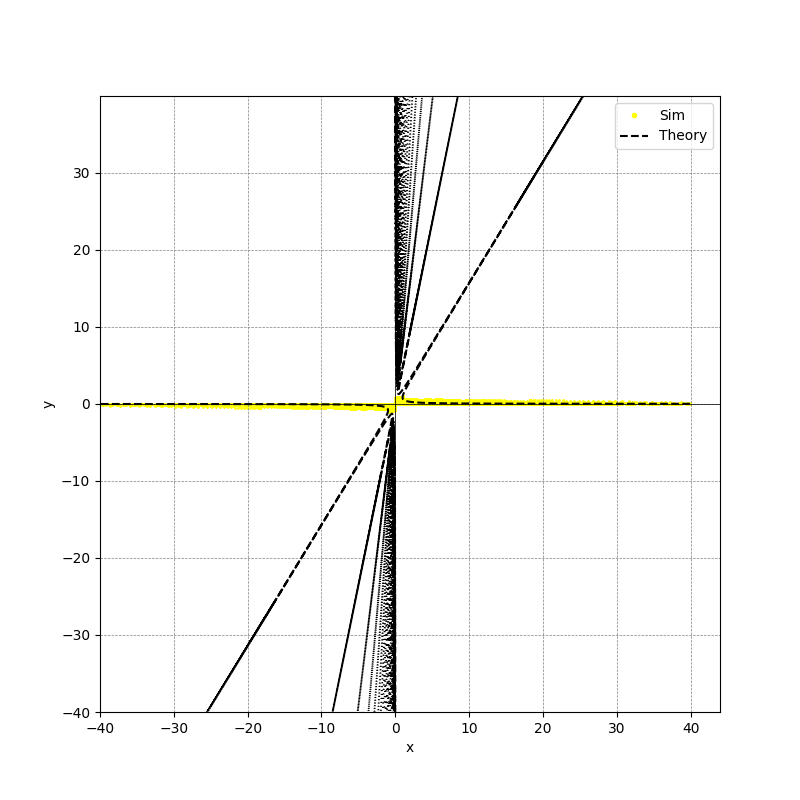
\includegraphics[width=0.8\linewidth]{figs/figb.png}
		\caption{}
		\label{graph3}
	\end{figure}
\end{frame}
\end{document}
